\documentclass[10pt]{article}
\usepackage[a4paper,margin=1.9cm]{geometry}
\usepackage{amsmath,amssymb}
\usepackage{graphicx}
\graphicspath{{../}{./}}
\usepackage{float}
\usepackage[dvipsnames]{xcolor}
\usepackage{enumitem}
\usepackage{titlesec}
\usepackage[hidelinks]{hyperref}

% --- compact layout ---
\setlist[itemize]{leftmargin=1.35em,itemsep=1pt,topsep=2pt,parsep=0pt}
\setlength{\parindent}{0pt}
\setlength{\parskip}{3pt}
\titlespacing*{\section}{0pt}{6pt}{3pt}
\titlespacing*{\subsection}{0pt}{4pt}{2pt}
\titleformat{\section}{\normalfont\large\bfseries\color{RoyalBlue}}{\thesection.}{0.5em}{}
\titleformat{\subsection}{\normalfont\bfseries}{}{0em}{}

\newcommand{\code}[1]{\texttt{\small #1}}
\newcommand{\file}[1]{\textcolor{RoyalBlue}{\texttt{\small #1}}}

% \docheader{title}{subtitle}
\newcommand{\docheader}[2]{%
  \begin{center}
    {\LARGE\bfseries #1}\\[2pt]
    {\small #2}
  \end{center}
  \vspace{-4pt}\hrule\vspace{6pt}
}

\begin{document}

\docheader{Adora --- CPU Performance \& Scaling}%
{1.5D Stokes synthesis benchmark \quad$\cdot$\quad Ivan Milic \quad$\cdot$\quad 2026-08-28 \quad$\cdot$\quad benchmark note}

\textbf{What was measured.} Column-by-column 1.5D full-Stokes synthesis (\file{synth3d.py}) of a
$100\times100$ atmosphere cube: a FALC column tiled across the map with velocity/field ramps, Fe\,\textsc{i}
630.15/630.25\,nm, $101$ wavelengths, $n_z=82$ depths --- i.e.\ $10^4$ independent columns, each a polarised
DELO solve through the differentiable stack. Hardware: a 256-core CPU node; env \code{adora-develop}
(JAX \code{0.7.1}, \code{fp64}). The engine is unchanged --- only \emph{how the columns are distributed}
across cores varies.

\subsection*{Headline: cost per pixel}
A ``pixel'' is one full column (all wavelengths, all four Stokes parameters). Single-device JAX runs one
column in \textbf{$\approx6.5$\,ms} but only reaches $\sim$8 effective cores --- most of XLA's CPU threads
\emph{spin-wait}, because this kernel exposes only $\sim$2 cores of real intra-instance parallelism.
Spreading the $10^4$ columns over independent, core-pinned worker processes collapses that to
\textbf{219\,µs\,/\,pixel} --- a \textbf{$\sim$30$\times$ speed-up} --- and genuinely uses the cores.

\begin{minipage}[t]{0.46\textwidth}
\vspace{2pt}
\subsection*{Process-parallel scaling ($100\times100$)}
Total core budget fixed at 64; workers pinned to disjoint core sets with \code{os.sched\_setaffinity},
launched via \code{multiprocessing} \code{spawn} from a JAX-free parent.

\smallskip
\begin{tabular}{@{}c c r r r r@{}}
\hline
\textbf{proc} & \textbf{core} & \textbf{comp.} & \textbf{run} & \textbf{µs/} & \textbf{eff.}\\
$\times$ & /proc & (s) & (s) & px & cores\\
\hline
$8$  & 8 & 11.5 & 10.51 & 1051 & 15.4\\
$16$ & 4 &  7.4 &  6.17 &  617 & 24.5\\
$32$ & 2 &  6.6 &  3.34 &  334 & 41.2\\
\textbf{64} & \textbf{1} & \textbf{6.4} & \textbf{2.19} & \textbf{219} & \textbf{55.7}\\
\hline
\end{tabular}

\smallskip
\code{run} = wall for one full $100\times100$ Stokes cube (concurrent workers); \code{comp.} is the one-time
JIT compile. All outputs finite and identical in shape $(100,100,4,101)$. \textbf{64 single-core processes
win}: 100$\times$100 in \textbf{2.2\,s} at \textbf{55.7/64 effective cores} (87\% efficiency). Fewer cores per
worker $\Rightarrow$ less spin-wait wasted $\Rightarrow$ near-linear scaling.
\end{minipage}\hfill
\begin{minipage}[t]{0.51\textwidth}
\vspace{0pt}
\begin{figure}[H]
  \centering
  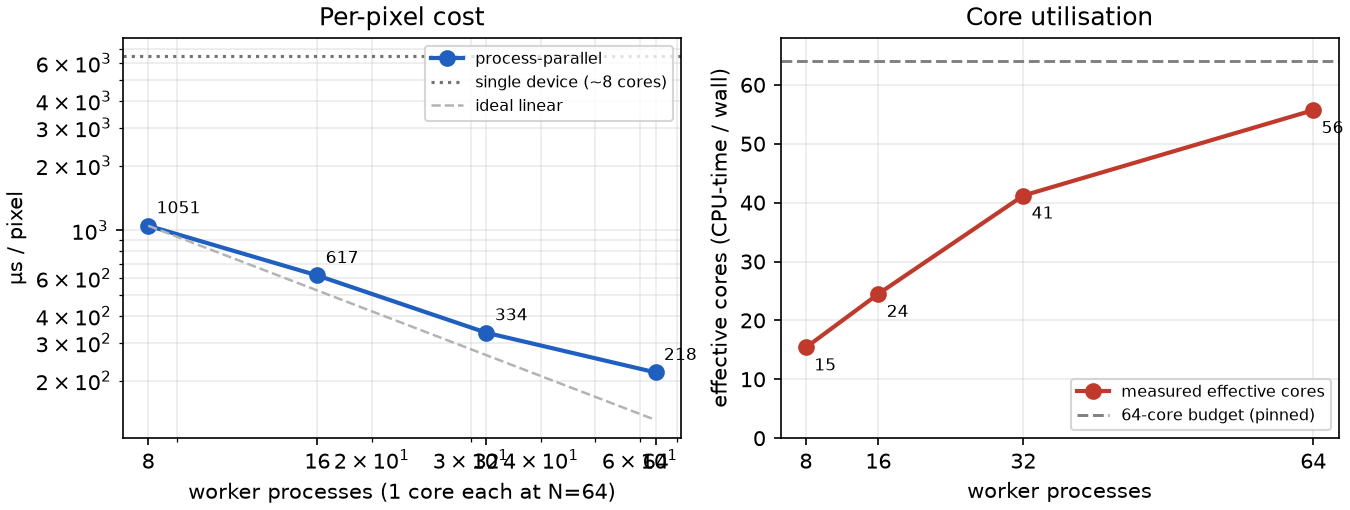
\includegraphics[width=\linewidth]{benchmark_scaling.png}
  \caption{\small \emph{Left:} per-pixel cost drops nearly linearly as the fixed 64-core budget is split into
  more, smaller workers, approaching the ideal; the single-device path (dotted) is $\sim$30$\times$ slower.
  \emph{Right:} measured effective cores climb toward the 64-core budget, reaching 55.7 at 64$\times$1.}
  \label{fig:scaling}
\end{figure}
\end{minipage}

\subsection*{What did \emph{not} work, and why}
\begin{itemize}
  \item \textbf{Single XLA device (default).} Auto-multithreads to only $\sim$8 effective cores on this kernel
        and can go no wider; the batch \code{vmap} over columns is not exposed as core-level parallelism.
  \item \textbf{\code{pmap} over 64 host CPU ``devices''.} Hit the 64-core target, but pathological:
        \textbf{366\,s} to compile the fused \code{fp64} program and \textbf{$>$200\,s} per run --- i.e.\
        \emph{slower per pixel than 8 cores}. Naive \code{pmap}-of-\code{vmap} is a dead end on XLA-CPU here.
  \item \textbf{Process-level data parallelism (the winner).} Independent single-device workers, one core
        each, pinned to disjoint cores. No giant fused kernel, 6\,s compile, near-linear scaling. The
        parent stays numpy-only so \code{spawn}'d workers start with a clean JAX.
\end{itemize}

\subsection*{Takeaways for the 3D extension}
\begin{itemize}
  \item Scale by \textbf{running many single-core column workers}, not by widening one XLA computation.
  \item \textbf{Projection:} at 219\,µs/px a real $512\times512$ snapshot ($2.6\times10^5$ columns)
        $\approx$\,\textbf{57\,s}/run + one $\sim$6\,s compile --- vs.\ $\sim$28\,min single-core.
  \item Next: fold a \code{synth\_cube\_mp(cube, waves, dz, nworkers)} helper beside \file{synth3d.py};
        GPU would sidestep the CPU spin-wait entirely (needs fast \code{fp64}).
\end{itemize}

\end{document}
